\documentclass[a4paper]{article}

\usepackage{../styles/new-style}
\usepackage{float}
\usepackage{tikz}

\newcommand{\hmwkTitle}{Lühimad teed graafis} % Assignment title
\newcommand{\hmwkClass}{Algoritmid ja andmestruktuurid} % Course/class

\begin{document}

\textbf{Kodutöö esitamise tähtaeg: 3. detsember, 23:59}

{\center
\subsection*{Graaf}
}

Graaf on abstraktne andmestruktuur, mis koosneb \textbf{tippudest}  (\textit{vertices}) ning nendevahelistest \textbf{servadest} (\textit{edges}).

\begin{figure}[H]
\centering
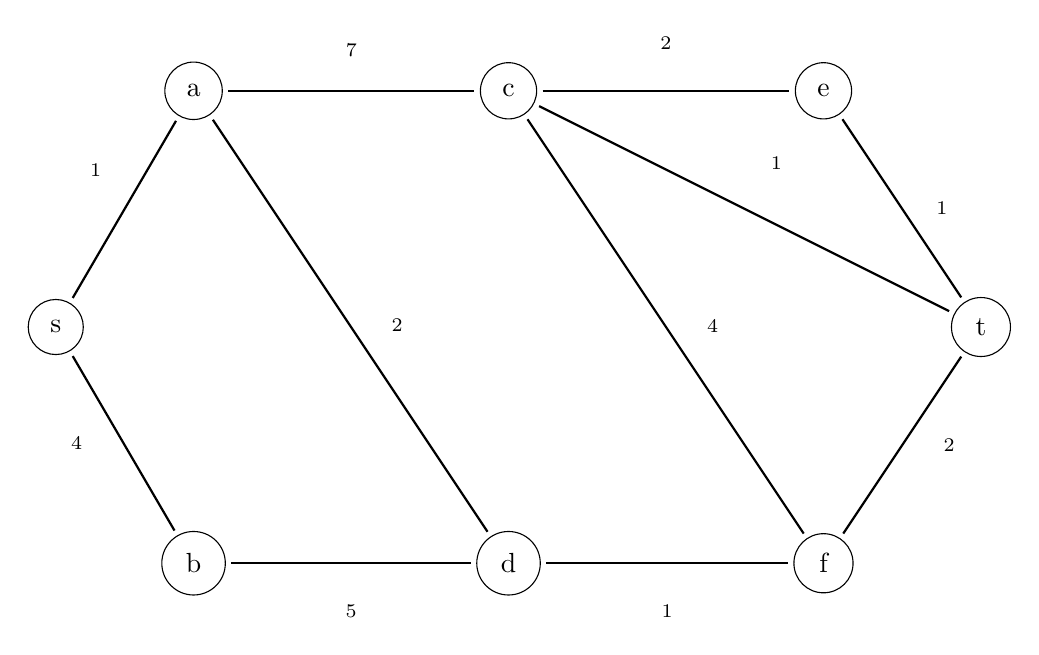
\begin{tikzpicture}
\node[shape= circle, draw, inner sep=5pt] (s) at (1.25,0) {s};
\node[shape = circle, draw, inner sep=5pt] (a) at (3,3) {a};
\node[shape = circle, draw, inner sep=5pt] (b) at (3,-3) {b};
\node[shape = circle, draw, inner sep=5pt] (c) at (7,3) {c};
\node[shape = circle, draw, inner sep=5pt] (d) at (7,-3) {d};
\node[shape = circle, draw, inner sep=5pt] (e) at (11,3) {e};
\node[shape = circle, draw, inner sep=5pt] (f) at (11,-3) {f};
\node[shape = circle, draw, inner sep=5pt] (t) at (13,0) {t};
\path[ thick, shorten <=2pt,shorten >=2pt, every node/.style={font=\scriptsize}]
(s) edge node[label={[label distance=5]120:$1$}] {} (a)
(f) edge node[label={[label distance=7.5]0:$2$}] {} (t)
(s) edge node[label={[label distance=7.5]180:$4$}] {} (b)
(e) edge node[label={[label distance=5]0:$1$}] {} (t)
(a) edge node[label={[label distance=5]90:$7$}] {} (c)
(b) edge node[label={[label distance=7.5]270:$5$}] {} (d)
(d) edge node[label={[label distance=7.5]0:$2$}] {} (a)
(d) edge node[label={[label distance=7.5]270:$1$}] {} (f)
(c) edge node[label={[label distance=7.5]90:$2$}] {} (e)
(c) edge node[label={[label distance=7.5]60:$1$}] {} (t)
(c) edge node[label={[label distance=7.5]0:$4$}] {} (f);
\end{tikzpicture}
\caption{Graaf}
\end{figure}

Graafi implementatsioonid põhinevad tavaliselt kas  \textbf{naabrusmaatriksil} (\textit{adjacency matrix}) või  \textbf{naabrusjärjenditel} (\textit{adjacency lists}).

Eelneva graafi naabrusmaatriks, kus $-1$ tähistab serva puudumist, on järgmine:

\begin{figure}[H]
\centering
\begin{tabular}{c | c c c c c c c r}
& s & a & b & c & d & e & f & t \\
\hline
s & -1 & 1 & 4 & -1 & -1 & -1  & -1 & -1 \\
a & 1 & -1 & -1 & 7 & 2 & -1  & -1 & -1 \\
b & 4 & -1 & -1 & -1 & 5 & -1  & -1 & -1 \\
c & -1 & 7 & -1 & -1 & -1 & 2  & 4 & 1 \\
d & -1 & 2 & 5 & -1 & -1 & -1  & 1 & -1 \\
e & -1 & -1 & -1 & 2 & -1 & -1  & -1 & 1 \\
f & -1 & -1 & -1 & 4 & 1 & -1  & -1 & 2 \\
t & -1 & -1 & -1 & -1 & -1 & 1  & 2 & -1 \\
\end{tabular}
\caption{Naabrusmaatriks}
\end{figure}

Paneme tähele, et kuigi see maatriks määrab üheselt ära graafi, siis arvestatav osa maatriksi väljadest tähistavad serva puudumist.

Eelneva graafi naabrusjärjendid on:

\begin{figure}[H]
\centering
\begin{tabular}{c | c c c c}
\hline
s & (s,a,1) & (s,b,4) & & \\
a & (s,a,1) & (a,c,7) & (a,d,2)  &  \\
b & (s,b,4) & (b,d,5) &  &  \\
c & (a,c,7) & (c,e,2) & (c,f,4) & (c,t,1) \\
d & (a,d,2) & (b,d,5) & (d,f,1) &   \\
e & (c,e,2) & (e,t,1) & &\\
f & (c,f,4) & (d,f,1) & (f,t,2) & \\
t & (c,t,1) & (e,t,1) & (f,t,2) &  \\
\end{tabular}
\caption{Naabrusjärjendid}
\end{figure}

Kasutades üht neist kahest ideest, lahendada järgmine ülesanne:

\begin{problem}
\textbf{Ülesanne 1 (40\%)}

Implementeerida graaf vastavalt liidesele \textit{Graph}.
\end{problem}

{\center
\subsection*{Lühimad teed graafis}
}

Sageli kasutame graafe nii, et servaga seotud väärtust võib tõlgendada kui kaugust kahe tipu vahel. Sellisel juhul tõuseb tihti esile järgnev probleem -- \textbf{leida lühima kaugusega teed graafi tipust $v$ kõikidesse teistesse graafi tippudesse}.

Loengus olete tutvunud mitme algoritmiga selle probleemi lahendamiseks: Floyd-Warhsalli algoritm, Bellman-Fordi algoritm ja Dijkstra algoritm. 

Kasutades üht kolmest ülalmainitud algoritmist, lahendada järgmine ülesanne. 60 \% saamiseks tuleb ülesanne lahendada Dijkstra algoritmi kasutades. Kasutades Floyd-Warhsalli või Bellman-Fordi algoritmi, on võimalik saada 40\%.

\begin{problem}
\textbf{Ülesanne 2 (40\% - 60\%)}

Implementeerida lühimate teede leidmise algoritm vastavalt liidesele \textit{ShortestPathsFromVertex}.
\end{problem}

Liidesed on kättesaadavad aaddressil \url{https://github.com/ut-aa/aa2016-lab7}.

\end{document}